\documentclass{../../oss-handout}
\usepackage{enumitem}
\usepackage{tikz}


\tikzset{
  >=latex
}

\setlength{\parindent}{0pt}
\setlength{\parskip}{8pt}
\setlength{\headheight}{26pt}


% Set the page style for the document
\pagestyle{plain}

% Course & handout information
\renewcommand{\institution}{Meritus Academy}
\renewcommand{\coursetitle}{Advanced Placement Physics C}
\renewcommand{\term}{Updated: Summer 2023}

\title{Example Multi-Body Dynamic Problems}
\author{Dr.\ Timothy Leung}
\date{\today}

\begin{document}
\thispagestyle{title}
\gentitle

\begin{center}
  \begin{tikzpicture}[thick]
     \draw (-1,0)--(12,0);
     \draw[fill=purple!40] rectangle (1.5,1) node[midway]{$m_3$};
     \draw (1.5,.5)--(3.5,.5) node[midway,above]{$T_2$};
     \draw[fill=purple!40] (3.5,0) rectangle (5,1) node[midway]{$m_2$};
     \draw (5,.5)--(7,.5) node[midway,above]{$T_1$};
     \draw[fill=purple!40] (7,0) rectangle (8.5,1) node[midway]{$m_1$};
     \draw[ultra thick,->] (8.5,.5)--(10.5,.5) node[right]{$\mathbf F$};  
  \end{tikzpicture}
\end{center}
Three masses, connected by massless ropes, are pulled forward by an external
force $\mathbf F$ over a frictionless surface.
\begin{enumerate}[nosep]
  \item What is the acceleration of the masses?
  \item What are the tension forces in the ropes?
\end{enumerate}
\newpage


\begin{center}
  \begin{tikzpicture}[thick]
     \draw (-3,0)--(6,0);
     \draw[fill=cyan!10] rectangle(1,1) node[midway]{$m_1$};
     \draw[fill=cyan!30] (1,0) rectangle(2.5,1.5) node[midway]{$m_2$};
     \draw[fill=cyan!50] (2.5,0) rectangle(4.3,1.8) node[midway]{$m_3$};
     \draw[ultra thick,->] (-1.5,.5)--(0,.5) node[pos=0,left]{$\mathbf F$};  
  \end{tikzpicture}
\end{center}
Three masses are pushed forward by an external force $\mathbf F$ over a
frictionless surface. What is the acceleration of the masses?
\newpage


\begin{center}
  \begin{tikzpicture}[thick]
    \draw (-1.5,0)--(5.5,0);
    \draw[fill=magenta!50] rectangle (3,1.5) node[midway]{$m_2$};
    \draw[fill=magenta!25] (.75,1.5) rectangle (2.25,2.5) node[midway]{$m_1$};
    \draw[ultra thick,->] (3,.8)--(4.5,.8) node[right]{$\mathbf F$};
  \end{tikzpicture}
\end{center}
Masses $m_1$ and $m_2$ are pulled forward by a external force $\mathbf F$
without slipping.
\begin{enumerate}[nosep]
  \item What is the \emph{maximum} acceleration that the masses can have without
  slipping?
  \item What is the magnitude of the external force at maximum acceleration?
\end{enumerate}
\newpage


\begin{center}
  \begin{tikzpicture}[thick]
    \draw circle (.5);
    \draw (0,0)--(0,1);
    \draw (.5,0)--(.5,-2);
    \draw (-.5,0)--(-.5,-3);
    \draw[fill=lightgray] (.2,-2) rectangle (.8,-2.6) node[below left]{$m$};
    \draw[fill=gray] (-.2,-3) rectangle (-.8,-4.2) node[below right]{$M$};
    \draw (-2,1)--(2,1);
  \end{tikzpicture}
\end{center}
Two masses ($M>m$) are connected by a massless string over a massless and
frictionless pulley. What is the magnitude of acceleration of the masses?
\newpage



%\begin{center}
%  \begin{tikzpicture}[scale=1.2,thick]
%    \draw[brown] (-4,.4)--(.1,.4);
%	\draw (0,0)--(-5.5,0) node[midway,below]{$\mu$};
%    \draw[fill=magenta!20] (-4,0) rectangle(-5,.75)node[midway]{$m$};
%    \begin{scope}[rotate=-30]
%      \draw[brown] (1,.4)--(-.05,.4);
%      \draw (0,0)--(3,0) node[midway,below left] {$\mu$};
%      \draw[fill=cyan!50] (1,0) rectangle(2.5,1)node[midway,rotate=-30]{$M$};
%    \end{scope}
%    \begin{scope}[rotate=-15]
%      \draw[fill=gray] (0,.3) circle(.15);
%      \draw[fill=lightgray] (0,.3) circle(.1);
%      \draw[ultra thick] (0,0)--(0,.3);
%      \fill(0,.3) circle(.04);
%    \end{scope}
%    \draw[gray!70] (0,0)--(0,-1.5);
%    \draw[->] (0,-.5)arc(270:330:.5) node[midway,below]{$\phi$};
%  \end{tikzpicture}
%\end{center}

\end{document}
